\documentclass[../main.tex]{subfiles}

\begin{document}

\section{Operations, Primitives and Algorithms}
The following sections introduce, define and explain Operations, Primitives and Algorithms generally using the Terminology presented below. Operations are the building blocks of Primitives whereas Primitives are the building blocks of Algorithms. The definitions which follow are flexible enough to support implementation across programing languages but have been inspired by the core concepts found within Lisp and Z. The focus of these sections is to define the properties of and interactions between Operations, Primitives and Algorithms in a general way which doesn't place unnecessary bounds on their range of possible functionality with respect to processing xAPI data.

\subsection{Terminology}

Within this document, (s) indicates one or more.
When talking about some $x \in X$ at some index within a range $i~..~n~..~j$, the notation $i_{x} ~\lor ~n_{x}, ~\lor ~j_{x}$ may be used in cases where it is a more concise version of an equivalant expression.

\subsubsection{Scalar}
When working with xAPI data, Statements are written using \href{https://www.json.org/}{JavaScript Object Notation} (JSON).
This data model supports a few fundamental types as described by \href{https://json-schema.org/understanding-json-schema/reference/type.html}{JSON Schema}.
In order to speak about a singular valid JSON value (string, number, boolean, null) generically, the term Scalar is used.
To talk about a scalar within a Z Schema, the following free and basic types are introduced.
\begin{zed}
  [STRING, NULL] \\
  Boolean :== true ~| ~false \\
  Scalar :== Boolean ~| ~STRING ~| ~NULL ~| ~\num
\end{zed}
Arrays and Objects are also valid JSON values but will be referenced using the terms Collection and Map respectively.

\subsubsection{Collection}
a sequence $\langle ... \rangle$ of items $c$ such that
\begin{axdef}
  C = \langle c_{i}..c_{n}..c_{j} \rangle \implies \{~i \mapsto c_{i}, n \mapsto c_{n}, j \mapsto c_{j} \}
  \where
  i \leq n \leq j \implies i \prec n \prec j \iff i \not= n \not= j
\end{axdef}
And the following free type is introducted for collections
\begin{argue}
  Collection :== emptyColl ~| ~append \ldata Collection \cross Scalar ~\lor Collection ~\lor Map \cross \nat \rdata \\
  \t1 emptyColl & the empty Collection $\langle  \rangle$ \\
  \t1 append & is a constructor and is infered to be an injection \\
  \t1 Map & a free type introduced bellow \\
  append(emptyColl, c?, 0) = \langle c_{0} \rangle \implies \{~0 \mapsto c?\}
\end{argue}

\subsubsection{Key}

An identifier $k$ paired with some value $v$ to create an ordered pair $(k, v)$. $k$ can take on any valid JSON value (Scalar, Collection, Map)
but the Scalar null should be avoided. The following free type is introduced for keys.
\begin{zed}
  K ::= Scalar ~| ~Collection ~| ~Map
\end{zed}

\subsubsection{Value}

A value $v$ is paired with an identifier $k$ to create an ordered pair $(k, v)$. $v$ can be any valid JSON value (Scalar, Collection, Map)
The following free type is introduced for values.

\begin{zed}
  V ::= Scalar ~| ~Collection ~| ~Map
\end{zed}

\subsubsection{Map}
Within the Z Notation Introduction section, Maps are introduced using the free type $KV$.
\begin{zed}
  KV ::= base ~| ~associate \ldata~KV \cross X \cross Y \rdata
\end{zed}
This definition is more accurately
\begin{zed}
  KV ::= base ~| ~associate \ldata~KV \cross K \cross V \rdata
\end{zed}
which indicates the usage of Key $k$ and Value $v$ within $associate$. Using this updated definition,
\begin{zed}
  associate(base, k, v) = \ldata (k, v) \rdata
\end{zed}
such that a Map is a Collection of ordered pairs $(k_{n}, v_{n})$ and thus a Collection of mappings
\begin{zed}
  (k_{n}, v_{n}) \implies k_{n} \mapsto v_{n}
\end{zed}
but Maps are special cases of Collections as $k_{n}$ is the unique identifier of $v_{n}$ within a Map
but the opposite is not true. In fact, keys are their own identifiers
\begin{zed}
  \id v_{n} = k_{n} \\
  \id k_{n} \not= v_{n} \\
  \id k_{n} = k_{n}
\end{zed}
Given a Map $M = \ldata (k_{i}, v_{i})~..~(k_{n}, v_{n})~..~(k_{j}, v_{j}) \rdata$ the following demonstrates the uniqueness of Keys
but the same is not true for all $v$ within $M$
\begin{zed}
  i_{k} \not= n_{k} \not= j_{k} \\
  i_{v} = n_{v} \lor i_{v} \not= n_{v} \
  i_{v} = j_{v} \lor i_{v} \not= j_{v} \
  j_{v} = n_{v} \lor j_{v} \not= n_{v}
\end{zed}
which can all be stated formally as
\begin{gendef}[K, V]
  Map : K \cross V \bij KV
  \where
  Map = \ldata (k_{i}, v_{i})~..~(k_{n}, v_{n})~..~(k_{j}, v_{j}) \rdata @ \\
  \t1 \dom Map = \{~ k_{i}~..~k_{n}~..~k_{j}\} \\
  \t1 \ran Map = \{~v_{i}~..~v_{n}~..~v_{j}\} \\
  \t1 first(k_{i}, v_{i}) \not= first(k_{n}, v_{n}) \not= first (k_{j}, v_{j}) ~\land \\
  \t1 i_{v} = n_{v} \lor i_{v} \not= n_{v} \ i_{v} = j_{v} \lor i_{v} \not= j_{v} \ j_{v} = n_{v} \lor j_{v} \not= n_{v} ~\land \\
  \t1 \id ~v_{i} = k_{i} ~\land \id ~v_{n} = k_{n} ~\land \id ~v_{j} = k_{j} ~\land \\
  \t1 \id ~k_{i} = k_{i} ~\land \id ~k_{n} = k_{n} ~\land \id k_{j} = k_{j}
\end{gendef}
Given that $v$ can be a Map $M$, or a Collection $C$, Arbitrary nesting is allowed within Maps but the properties of a Map hold at any depth.
$$M = \ldata (k_{i}, v_{i})~..~(k_{n}, \ldata (k_{ni}, v_{ni}) \rdata)~..(k_{j}, \langle v_{ji}~..~\ldata (k_{jn}, v_{jn}) \rdata~..~\langle v_{jji}~..~v_{jjn}~..~v_{jjj}\rangle\rangle) \rdata$$
such that $\ldata (k_{ni}, v_{ni}) \rdata$ and $\ldata (k_{nj}, v_{nj}) \rdata$ are both Maps and adhere to the constraints enumerated above.

\subsubsection{Statement}

Immutable Map conforming to the \href{https://github.com/adlnet/xAPI-Spec/blob/master/xAPI-Data.md#24-statement-properties}{xAPI Specification} as described in the xAPI Formal Definition section of this document. The imutability of a Statement $s$ is demonstrated by the following
which indicates that $s$ was not altered when passed to $associate$.
\begin{axdef}
  s!, s? : STATEMENT \\
  k? : K \\
  v? : V \\
  \where
  s! = associate(s?, k?, v?) = s? \implies (k?, v?) \not \in s! \implies s! = s? \\
\end{axdef}
 Additionally, given the schema $Statements$ the following is true for all $Statement$(s)
\begin{axdef}
  Statements \\
  Keys : STRING \\
  S : Collection
  \where
  Keys = \{~id, actor, verb, object, result, context, attachments, timestamp, stored\} \\
  \dom statement = K \dres Keys \\
  S = \langle ~statement_{i}~..~statement_{n}~..~statement_{j} \rangle @ \\
  \t1 atKey(statement_{i}, id) \not= atKey(statement_{n}, id) \not= atKey(statement_{j}, id) \implies \\
  \t1 id_{i} \not= id_{n} \not= id_{j} \iff statement_{i} \not= statement_{n} \not= statement_{j}
\end{axdef}
Which confirms the constraints found in the schema $Statement$ and adds an additional constraint
to $Statements$ such that every unique $Statement$ in a $Collection$ of $Statements$ has a unique $id$.

\subsubsection{Algorithm State}

Mutable Map $state$ without any domain restriction such that
\begin{axdef}
  state?, state! : Map \\
  k? : K \\
  v? : V
  \where
  associate(state?, k?, v?) = state! @ (k, v) \in state! \implies state? \not= state!
\end{axdef}

\subsubsection{Option}

Mutable Map $opt$ which is used to alter the result of an Algorithm. The effect of $opt$ on an Algorithm will be discussed in the Algorithm Result section bellow.

\section{Operation}

An Operation is a function of arbitrary arguments and is defined using Z. For example, Operations pulled directly from "The Z Notation: A Reference Manual" include
\begin{itemize}
\item $first$
\item $second$
\item $succ$
\item $\min$
\item $\max$
\item $count \equiv \#$
\item $\cat$
\item $rev$
\item $head$
\item $last$
\item $tail$
\item $front$
\item $\extract$
\item $\filter$
\item $\dcat$
\item $\disjoint$
\item $\partition$
\item $\otimes$
\item $\uplus$
\item $\uminus$
\item $items$
\end{itemize}

\subsection{Domain}
The arguments passed to an Operation can be any of the following but the definition of an Operation may limit the domain to a subset of the following
\begin{itemize}
\item Key(s)
\item Value(s)
\item Set(s)
\item Collection(s)
\item Bag(s)
\item Map(s)
\item Statement(s)
\item Algorithm State
\end{itemize}

\subsection{Range}
The result of an Operation can be any of the following but the definition of an Operation may limit this range to a subset of the following

\begin{itemize}
\item Key(s)
\item Value(s)
\item Set(s)
\item Collection(s)
\item Bag(s)
\item Map(s)
\item Statement(s)
\item Algorithm State
\end{itemize}

\section{Primitive}
A collection of Operations where the output of an Operation $o$ is passed as an argument to the next Operation.
\begin{zed}
  p_{\langle i~..~n~..~j \rangle} = o_{i} ~\pipe ~o_{n} ~\pipe ~o_{j}
\end{zed}
Within any given Primitive $p$, variables local to $p$ and any global variables may be passed as arguments to any $o$ within $p$ and there is no restriction on the ordering of arguments with respect to the piping. In the following, $q?$ is a global variable where as the rest are local.
\begin{axdef}
  x?, y?, z?, i!, n!, j!, p! : Value \\
  o_{i} : Value \fun Value \\
  o_{n} : Value \cross Value \fun Value \\
  o_{j}, p : Value \cross Value \cross Value \fun Value \\
  \where
  i! = o_{i}(x?) \\
  n! = o_{n}(i!, y?) \\
  j! = o_{j}(z?, n!, q?) \\
  p! = j! \implies o_{j}(z?, o_{n}(o_{i}(x?), y?), q?)
\end{axdef}
Primitives break the processing of xAPI data down into discrete units that can be composed to create new analytical functions. Primitives allow users to address the methodology of answering research questions as a sequence of generic algorithmic steps which establish the necessary data transformations, aggregations and calculations required to reach the solution in an implementation agnostic way.

\subsection{Domain}
Any of the following dependent upon the Operations which compose the Primitive

\begin{itemize}
\item Key(s)
\item Value(s)
\item Set(s)
\item Collection(s)
\item Bag(s)
\item Map(s)
\item Statement(s)
\item Algorithm State
\end{itemize}

\subsection{Range}
Any of the following dependent upon the Domain and Functionality of the Primitive

\begin{itemize}
\item Key(s)
\item Value(s)
\item Set(s)
\item Collection(s)
\item Bag(s)
\item Map(s)
\item Statement(s)
\item Algorithm State
\end{itemize}

\section{Algorithm}
Given a Collection of statement(s) $S_{<a..b..c>}$ and potentially option(s) $opt$ and potentially an existing Algorithm State $state$ an Algorithm $A$ executes as follows

\begin{enumerate}
\item call $init$
\item for each $stmt \in S_{<a..b..c>}$
  \begin{enumerate}
  \item $relevant?$
  \item $accept?$
  \item $step$
  \end{enumerate}
\item return $result$
\end{enumerate}
with each process within $A$ is enumerated as

\begin{lstlisting}[frame=single]
  (init [state] body)
   - init state

  (relevant? [state statement] body)
   - is the statement valid for use in algorithm?

  (accept? [state statement] body)
   - can the algorithm consider the current statement?

  (step [state statement] body)
   - processing per statement
   - can result in a modified state

  (result [state] body)
   - return without option(s) provided
   - possibly sets default option(s)

  (result [state opt] body)
   - return with consideration to option(s)
\end{lstlisting}
\begin{itemize}
\item $body$ is a collection of Primitive(s) which establishes the processing of inputs $\to$ outputs
\item $state$ is a mutable Map of type $KV$ and synonymous with Algorithm State
\item $statement$ is a single statement within the collection of statements passed as input data to the Algorithm $A$
\item $opt$ are additional arguments passed to the algorithm $A$ which impact the return value of the algorithm and synonymous with Option
\end{itemize}
Such that the execution of A can be described as
\begin{zed}
  Algorithm ::= Init \semi Relevant? \semi Accept? \semi Step \semi Result
\end{zed}
\subsection{Domain}
An Algorithm must be passed an Algorithm State and a Collection of Statement(s). Option is optional.
\begin{itemize}
\item Statement(s)
\item Algorithm State
\item Option(s)
\end{itemize}

\subsection{Range}
An Algorithm will return an Algorithm State.
\begin{itemize}
\item Algorithm State
\end{itemize}

\subsection{Initialization}

First process to run within an Algorithm which returns the Algorithm State for the current iteration.

\begin{schema}{Init[KV]}
  state?, state! : KV \\
  init: KV \fun KV
  \where
  state! = init(state?) @ state! = state? ~\lor ~state! \not = state?
\end{schema}
such that some $state!$ does not need to be related to its arguments $state?$
but $state!$ could be derived from some seed $state?$.
This functionality is dependent upon the $body$ of an Algorithms $init$

\subsubsection{Domain}

\begin{itemize}
\item Algorithm State
\end{itemize}

\subsubsection{Range}

\begin{itemize}
\item Algorithm State
\end{itemize}

\subsection{Relevant?}

First process that each $stmt$ passes through such that
$$relevant? \prec accept? \prec step$$
resulting in an indication of whether the $stmt$ is valid for use within algorithm $A$
$$relevant?(state, stmt) = true \ \lor false$$
The criteria which determines validity of $stmt$ within $A$ is defined by the $body$ of $relevant?$

\subsubsection{Domain}

\begin{itemize}
\item Statement
\item Algorithm State
\end{itemize}

\subsubsection{Range}

\begin{itemize}
\item Scalar
\end{itemize}

\subsection{Accept?}

Second process that each $stmt$ passes through such that
$$relevant? \prec accept? \prec step$$
resulting in an indication of whether the $stmt$ can be sent to $step$ given the current $state$
$$accept?(state, stmt) = true \ \lor false$$
The criteria which determines usability of $stmt$ given $state$` is defined by the $body$ of $accept?$

\subsubsection{Domain}

\begin{itemize}
\item Statement
\item Algorithm State
\end{itemize}

\subsubsection{Range}

\begin{itemize}
\item Scalar
\end{itemize}

$\\\\\\$

\subsection{Step}

An Algorithm Step consists of a collection of Primitive(s) and therefore collection(s) of Operation(s)

\begin{figure*}[h]
  \centering
  {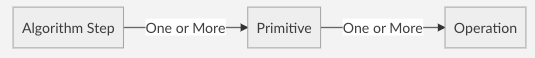
\includegraphics[scale=0.70]{algorithm-step-flat}}
\end{figure*}
$\\$
which expands to

\begin{figure*}[h]
  \centering
  {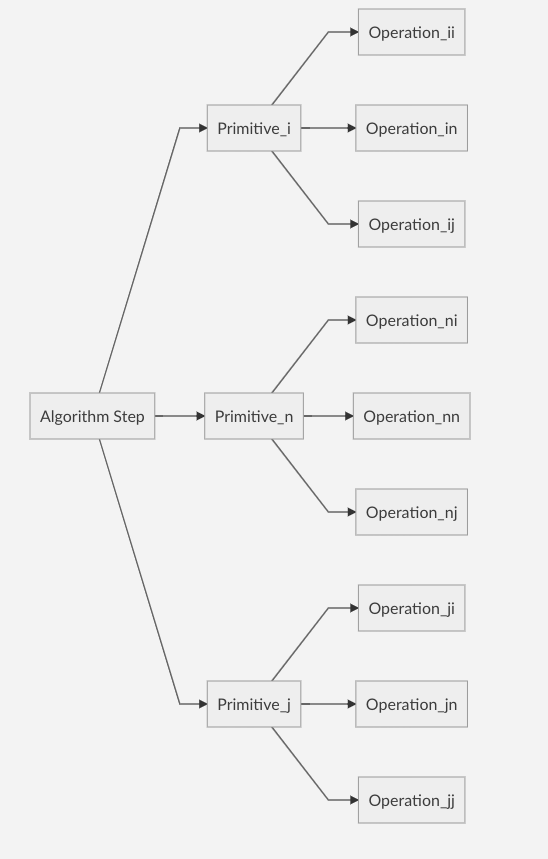
\includegraphics[scale=0.401]{algorithm-step-expanded}}
\end{figure*}
$$ i \leq n \leq j \implies i \prec n \prec j$$
$$ i_{i} \leq i_{n} \leq i_{j} \leq n_{i} \leq n_{n} \leq n_{j} \leq j_{i} \leq j_{n} \leq j_{j} \implies i_{<i..n..j>} \prec n_{<i..n..j>} \prec j_{<i..n..j>}$$
$\\$
where the output of a Primitive is passed as the argument to the next Primitive

\begin{figure*}[h]
  \centering
  {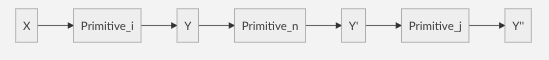
\includegraphics[page=1]{algorithm-step-args}}
\end{figure*}
$\\$
The selection and ordering of Operation(s) and Primitive(s) into an Algorithmic Step determines how the Algorithm State changes during iteration through Statement(s) passed as input to the Algorithm.

\subsubsection{Domain}

\begin{itemize}
\item Statement
\item Algorithm State
\end{itemize}

\subsubsection{Range}

\begin{itemize}
\item Algorithm State
\end{itemize}

\subsubsection{Formal Definition}

A collection of Primitive(s)

$$P = <p_{i}..p_{n}..p_{j}> $$
where

$$i \leq n \leq j \implies i \prec n \prec j \iff i \not= n \not= j$$
and

$$Z_{i} =p_{i}(Args) \implies O_{ij}(O_{in}(O_{ii}(Args)))$$
where

$$ii \leq in \leq ij \implies ii \prec in \prec ij \iff ii \not= in \not= ij$$
such that for each $stmt_{b}$ within a collection of Statement(s) $S$ defined as

$$ S = <stmt_{a}..stmt_{b}..stmt_{c}> $$
where

$$a \leq b \leq c \implies a \prec b \prec c \iff a \not= b \not= c$$
$\\\\\\$
and

$$a \not \mapsto i \ \land b \not \mapsto n \ \land c \not \mapsto j$$
The output of $step$ given a $stmt_{b}$ and $state_{b}$ is defined as

$$step(state_{b}, stmt_{b}) = p_{j}(p_{n}(Z_{ib}))$$
where

$$Z_{ib} = p_{i}(Args) \implies p_{i}(state_{b}, stmt_{b}) \implies O_{ij}(O_{in}(O_{ii}(state_{b}, stmt_{b})))$$
and subsequently

$$Z_{nb} = p_{n}(Z_{ib})$$
which establishes that

$$Z_{jb} = p_{j}(Z_{nb}) \implies p_{j}(p_{n}(p_{i}(state_{b}, stmt_{b})))$$
$\\$
such that for a given $stmt_{b}$, $P_{<i..n..j>}$ will always result in a $Z_{jb}$ but

$$ Z_{ib} = state_{b} \lor state'_{ib} \iff state_{b} \not = state'_{ib}$$
which means

$$Z_{nb} = p_{n}(state_{b}, stmt_{b}) \lor p_{n}(state'_{ib}, stmt_{b})$$
$$ \implies$$
$$Z_{nb} = state_{b} \ \lor state'_{ib} \ \lor state'_{nb}$$
$$\implies$$
$$Z_{nb} = Z_{ib} \lor state'_{nb} \ \iff \ state_{b} \not= state'_{ib} \not= state'_{nb} $$
and concludes with
$$Z_{jb} = p_{j}(state_{b}, stmt_{b}) \lor p_{j}(state'_{ib}, stmt_{b}) \lor p_{j}(state'_{nb}, stmt_{b})$$
$$\implies$$
$$Z_{jb} = state_{b} \lor state'_{ib} \lor state'_{nb} \lor state'_{jb}$$
$$\implies$$
$$Z_{jb} = Z_{nb} \lor state'_{jb}
\ \iff \
state_{b} \not= state'_{ib} \not= state'_{nb} \not= state'_{jb} $$

$\\\\\\$
such that

$$Z_{jb} \equiv state'_{b}$$
$$\implies$$
$$state'_{b} = state_{b} \lor state'_{ib} \lor state'_{nb} \lor state'_{jb}
\ \iff \
state_{b} \not= state'_{ib} \not= state'_{nb} \not= state'_{jb}$$
$\\$
the impact being that iteration through all $stmt \in S{<a..b..c>}$ results in a return of $Z_{jc}$ such that

$$Z_{ja} = step(state_{a}, stmt_{a})
\ \implies \
state'_{a} \equiv Z_{ja} = state_{a} \lor state'_{ia} \lor state'_{na} \lor state'_{ja} $$
and
$$Z_{jb} = step(Z_{ja}, stmt_{b})
\ \implies \
state'_{b} \equiv Z_{jb} = Z_{ja} \lor state'_{ib} \lor state'_{nb} \lor state'_{jb} $$
meaning
$$Z_{jc} = step(Z_{jb}, stmt_{c})
\ \implies \
state'_{c} \equiv Z_{jc} = Z_{jb} \lor state'_{ic} \lor state'_{nc} \lor state'_{jc}$$
such that each $stmt \in S{<a..b..c>}$ may not result in a mutation of $state$ from $state \to state'$
$$state'_{c} = Z_{jc}$$
$$\implies$$
$$state'_{c} = state_{a} \lor state_{ia} \lor state'_{na} \lor state'_{ja} \lor state'_{ib} \lor state'_{nb} \lor state'_{jb} \lor state'_{ic} \lor state'_{nc} \lor state'_{jc}$$
$$\implies$$
$$state'{c} = state_{a} \lor state'{c} \not= state{a}$$
$\\$
The no-op scenario described above is only a possibility of $step(state_{a}, stmt \in S_{<a..b..c>})$ but can be predicted to occur given
\begin{itemize}
\item The definition of individual Operations $O$ which constitute a Primitive $p$
  $$Operation(X) = Y \land Operation(X') = Y' \implies Y = Y' \iff X = X'$$
\item The ordering of $O_{<i..n..j>}$ within $p$
  $$i \prec n \prec j$$
\item The Primitive(s) $p$ chosen for inclusion within $P_{<i..n..j>}$
  $$Z_{i} =p_{i}(Args) \implies O_{ij}(O_{in}(O_{ii}(Args)))$$
  $$Z_{j} =p_{j}(Args) \implies O_{jj}(O_{jn}(O_{ji}(Args)))$$
  $$\forall Args \ \exists \ Z_{i} = Z_{j} \iff O_{ij}(O_{in}(O_{ii}(Args))) \equiv O_{jj}(O_{jn}(O_{ji}(Args)))$$
  $$<p_{i}, p_{j}> \equiv <p_{j}, p_{i}> \iff Z_{i} = Z_{j}$$
\item The ordering of $p \in P_{i..n..j}$ which implies the ordering of $O \in p_{<i..n..j>} \in P_{<ii..ij..ni..nj..ji..jj>}$
  $$i \prec n \prec j \implies ii \prec in \prec ij \implies ii \prec ij \prec ni \prec nj \prec ji \prec jj$$
  $$P_{i..n..j} = P_{x..y..z} \implies <p_{i}, p_{n}, p_{j}> \equiv <p_{x}, p_{y}, p_{z}> \iff p_{i} \equiv p_{x} \ \land \ p_{n} \equiv p_{y} \ \land \ p_{j} \ \equiv p_{z}$$
  $$\implies$$
  $$P_{i..n..j} = P_{x..y..z} \iff i \mapsto x \ \land \ n \mapsto y \ \land \ j \mapsto z \ \land \ Z_{i} = Z_{x} \ \land \ Z_{n} = Z_{y} \ \land \ Z_{j} = Z_{z}$$
\item The Key Value pair(s) $kv \in$ $stmt$ $\in S_{<a..b..c>}$
\item The ordering of Statement(s) $stmt \in S_{<a..b..c>}$ such that $a \prec b \prec c$
\end{itemize}

\subsection{Result}

Last process to run within an Algorithm which returns the Algorithm State $state$ without preventing subsequent call of $A$
$$relevant? \prec accept? \prec step \prec result \prec relevant? \iff S \not= \emptyset$$
$$\implies$$
$$relevant? \prec accept? \prec step \prec result \iff S = \emptyset$$
$\\$
such that if $S(t_{n}) = \emptyset$ and at some future point $j$ within the timeline $i..n..j$ this is no longer true $S(t_{j}) \not= \emptyset$ then
$$A(state_{n-1}, \ S(t_{n - 1})) = state_{n} = A(init(), \ S(t_{n - i})) \iff A(state_{n},\ S(t_{n})) = state_{n}$$
$\\$
such that the statement(s) added to $S$ between $t_{i}$  and $t_{n}$ is
$$S(t_{n - i})$$
and the statement(s) added to $S$ between $t_{n}$  and $t_{j}$ be
$$S(t_{j - n})$$
such that
$$ S(t_{n - i}) \ \cup \ S(t_{j - n}) = S(t_{j - i})$$
which means
$$ A(init(), \  S(t_{j - i})) = state_{j}$$
and establishes that $A$ can pick up from a previous $state_{n}$ without losing track of its own history.
$$A(result(state_{n}), \ S(t_{j-n})) = A(init(),\ S(t_{j - i})) = state_{j}$$
$$\iff$$
$$result(state_{n}) = A(init(),\ S(t_{n - i})) = state_{n}$$
$\\$
Which makes $A$ capable of taking in some $S_{<i..n..j..\infty>}$ as not all $s \in S_{<i..\infty>}$ have to be considered at once. In other words, the input data does not need to persist across the history of $A$, only the effect of $s$ on $state$ must be persisted.
$\\\\$
Additionally, the effect of $opts$ is determined by the $body$ within $result$ such that
$$A(result(state_{n}), \ S(t_{j-n}), \ opts)$$
$$\equiv$$
$$A(init(),\ S(t_{j - i}))$$
$$\equiv$$
$$A(init(),\ S(t_{j - i}), \ opts)$$
$$\equiv$$
$$A(result(state_{n}), \ S(t_{j-n}))$$
Which implies that $opts$ may have an effect on $state$ but not in a way which prevents backwards compatibility of $state$

\subsubsection{Domain}

\begin{itemize}
\item Algorithm State
\item Option(s)
\end{itemize}

\subsubsection{Range}

\begin{itemize}
\item Algorithm State
\end{itemize}

\end{document}
